\subsection{Criteria}
Due to the conditions this system is developed under flaws are to be expected. 
To minimize the amount of critical flaws the criteria \citep[p.~180]{Rod-Aalborg} upon which the system will be judged have been prioritized.
The idea is that development will be focused on the very important and important criteria to make sure that all of these work.
Less effort will be put into the less important, irrelevant or easily fulfilled criteria, making flaws in these areas more likely.
However, as established they are less important and therefore the flaws will most likely not be critical.
These priorities can be found in \cref{fig:criteria}.


%\begin{figure}[H]
%	\centering
%	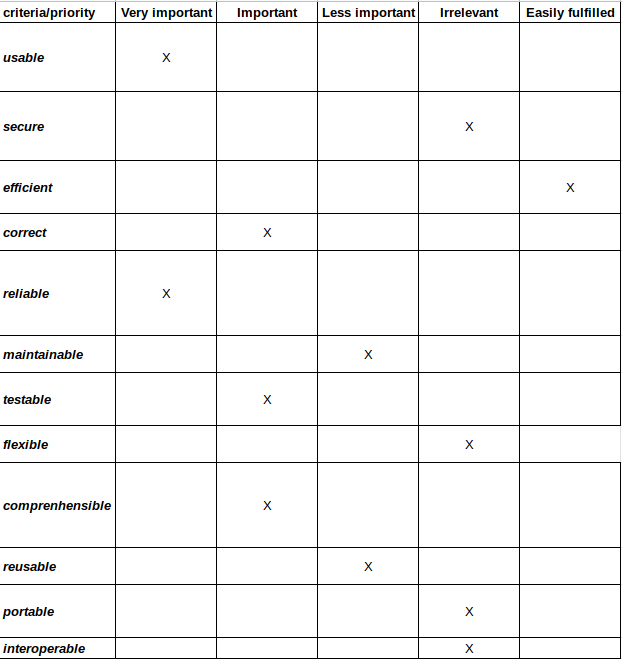
\includegraphics[width=1\textwidth]{billeder/architecture-priorities.png}
%	\caption{\textit{Prioritized list
%	}\label{fig:criteria}}
%\end{figure}
%Anna: Har lavet figuren om til en tabel nedenfor

\begin{table}[H]
	\begin{center}
		\begin{tabular}{|l|c|c|c|c|c|}
			\hline
			Criteria $\backslash$ priority & \rotatebox{90}{Very important} &  \rotatebox{90}{Important} & \rotatebox{90}{Less important} & \rotatebox{90}{Irrelevant} & \rotatebox{90}{Easily fulfilled}\\
			\hline
			Usable & \xmark & & & & \\
			\hline
			Secure & & & & \xmark & \\
			\hline
			Efficient & & & & & \xmark \\
			\hline
			Correct & & \xmark & & & \\
			\hline
			Reliable & \xmark & & & & \\
			\hline
			Maintainable & & & \xmark & & \\
			\hline
			Testable & & \xmark & & & \\
			\hline
			Flexible & & & & \xmark & \\
			\hline
			Comprehensible & & \xmark & & & \\
			\hline
			Reusable & & & \xmark & & \\
			\hline
			Portable & & & & \xmark & \\
			\hline
			Interoperable & & & & \xmark & \\
			%Anna: Hvad betyder det(er det stavet rigtigt)?
			\hline
		\end{tabular}
	\end{center}
	\caption{Prioritized list}\label{fig:criteria}
\end{table}


It is very important that the system is \textbf{usable}. It is assumed that the system will mainly have one user: The administrator. This fact could make this criterion less critical, however it is also assumed that this one user will have limited IT experience. Moreover this system is developed specifically for that one specific user and it is therefore imperative that they are able to use the system.

The user has expressed that whether or not the system is \textbf{secure} is no major concern as the information is not confidential. It has therefore been determined that security is outside this systems area of responsibility and it is prioritized as being irrelevant.

If compared to the existing solution to the problem making an \textbf{efficient} system is easily fulfilled as the existing solution is incredibly inefficient. The exact time it takes is less of a concern to the user.

Whether the system is \textbf{correct}, correct here used in the sense of it fulfils the system definition and meets all the requirements is important. The reasoning behind this not being very important is that there is a long list of requirements and they are not all equally necessary.

It is very important that the system is \textbf{reliable} as it is a massive problem for the user if the system malfunctions and eg. deletes files, assigns wrong version numbers or automatically approves a new version. Should any of these happen it could mean that the company will lose their certification which as described in \cref{sec:standards} is at best a problem for consumer trust and at worst a requirement by law.

Whether the system is \textbf{maintainable} is less important as the user won't be capable of maintaining it anyway.
 
The system needs to be \textbf{testable} in order to verify that it is reliable. Therefore this is important.



To summarize the prioritized criteria are the systems usability and reliability. Less important but still notable are correctness, testability and comprenhensibility. These criteria will therefore be prioritized when designing the components the system is made up of. 